\chapter{Caliente y frío}\label{ch:g1:hot-and-cold}

La sopa humea, el helado da dolor de dientes y el asiento del coche en
verano abrasa las piernas. Lo caliente y lo frío están por todas
partes. En este capítulo aprendemos a compararlos, a ver qué calienta
las cosas --- y a mirar qué le pasa a un cubito de hielo cuando gana
el calor.

\section{Más caliente y más frío}

\begin{definition}[Caliente y frío]\label{def:g1:hot-and-cold:words}
\emph{Caliente}\index{caliente} y \emph{frío}\index{frío} son palabras
que comparan, como grande y pequeño. La sopa está caliente
\emph{comparada con} tu mano; el hielo está frío \emph{comparado con}
tu mano. Entre las dos hay toda una escalera de palabras: helado,
frío, fresco, templado, tibio, caliente, ardiendo.
\end{definition}

\begin{omfigure}
\begin{tikzpicture}[scale=0.85]
  \draw[-Stealth, very thick] (0,0) -- (11.2,0);
  \node[below, font=\small] at (0.6,-0.25) {cubito de hielo};
  \node[below, font=\small] at (3.2,-0.25) {agua fresca};
  \node[below, font=\small] at (5.7,-0.25) {mi mano};
  \node[below, font=\small] at (8.2,-0.25) {sopa caliente};
  \node[below, font=\small] at (10.4,-0.25) {llama};
  \fill[omDef] (0.6,0) circle (2.6pt);
  \fill[omDef] (3.2,0) circle (2.6pt);
  \fill[omMeth] (5.7,0) circle (2.6pt);
  \fill[omThm] (8.2,0) circle (2.6pt);
  \fill[omThm] (10.4,0) circle (2.6pt);
  \node[above, font=\small] at (1.2,0.3) {más frío};
  \node[above, font=\small] at (9.9,0.3) {más caliente};
\end{tikzpicture}

{\small Una escalera del frío al calor: cada cosa encuentra su sitio,
con tu mano en algún punto del medio.}
\end{omfigure}

\begin{example}[Ordenar tres bebidas]\label{ex:g1:hot-and-cold:drinks}
En la mesa: un chocolate caliente, un vaso de agua del grifo y un vaso
de zumo de naranja recién sacado del frigorífico. Del más frío al más
caliente: el zumo, después el agua del grifo, después el chocolate. El
agua del grifo está fría al lado del chocolate y templada al lado del
zumo --- las palabras que comparan trabajan siempre por parejas.
\end{example}

\begin{remark}[Al tacto se le puede engañar]\label{rem:g1:hot-and-cold:fooled}
Acuérdate de los tres cuencos del capítulo anterior: la misma agua
templada le parecía caliente a una mano y fresca a la otra. Y toca una
cuchara de metal y otra de madera que hayan pasado la noche en la
misma cocina: la de metal se \emph{nota} más fría, aunque en la cocina
nada esté más frío que lo demás. El tacto es un guardián muy útil,
pero no es un juez justo --- muy pronto necesitaremos un instrumento
al que no se pueda engañar: el termómetro, que llega en un capítulo
posterior.
\end{remark}

\begin{method}[Comparar el calor y el frío con justicia]\label{met:g1:hot-and-cold:compare}
Para decidir cuál de dos cuencos de agua está más caliente:
\begin{enumerate}
  \item usa la \emph{misma} mano para los dos --- dos manos pueden no
        estar de acuerdo;
  \item toca uno y enseguida el otro --- si esperas, las cosas
        cambian;
  \item para estar aún más seguro, pide a un amigo que lo pruebe
        también, sin decirle antes tu respuesta.
\end{enumerate}
Si tu amigo y tú coincidís, la \omterm{def:g1:five-senses:observation}{observación} es firme.
\end{method}

\section{Qué calienta las cosas}

\begin{example}[Cosas que calientan]\label{ex:g1:hot-and-cold:warmers}
Algunas cosas calientan lo que tienen cerca: el Sol calienta el banco
del parque, la llama calienta la sartén, el radiador calienta la
habitación y tu propio cuerpo calienta la manta. Incluso frotar
calienta: junta las palmas de las manos y frótalas deprisa mientras
cuentas hasta $10$ --- nota cómo se calientan.
\end{example}

\begin{omfigure}
\begin{tikzpicture}[scale=0.8]
  % the sun, high on the left
  \fill[omThm] (1.0,3.3) circle (0.5);
  \foreach \a in {0,30,...,330} {
    \draw[omThm, thick] (1.0,3.3) ++(\a:0.68) -- ++(\a:0.32);
  }
  % ground line
  \draw[thick] (2.6,0) -- (11.6,0);
  % sunny bench, with two sun rays reaching it
  \draw[omThm] (1.55,2.95) -- (4.3,0.75);
  \draw[omThm] (1.75,3.1) -- (5.7,0.75);
  \draw[thick] (3.6,0.55) -- (6.4,0.55);
  \draw[thick] (3.8,0.55) -- (3.8,0) (6.2,0.55) -- (6.2,0);
  \node[below, font=\small] at (5.0,-0.15) {banco al sol: templado};
  % tree whose shade covers the second bench
  \draw[thick, fill=omExo!60] (8.05,0) rectangle (8.35,1.5);
  \draw[thick, fill=omMeth!45] (8.2,2.15) circle (0.95);
  \fill[omExo, opacity=0.3] (9.8,0.06) ellipse (1.75 and 0.2);
  \draw[thick] (8.6,0.55) -- (11.2,0.55);
  \draw[thick] (8.8,0.55) -- (8.8,0) (11.0,0.55) -- (11.0,0);
  \node[below, font=\small] at (9.9,-0.15) {banco a la sombra: fresco};
\end{tikzpicture}

{\small Dos bancos del mismo parque, el mismo día. El que recibe el
Sol está más caliente --- pruébalo con la mano un día soleado.}
\end{omfigure}

\begin{example}[Pruébalo: sol y sombra]\label{ex:g1:hot-and-cold:sunshade}
Un día soleado, pon una mano en una pared donde dé el sol y la otra en
la misma pared, a la sombra. Misma pared, mismo día --- pero el lado
del sol está claramente más caliente. El Sol es el gran calentador de
todo lo que hay al aire libre; pronto tendrá un capítulo entero para
él.
\end{example}

\begin{remark}[Los abrigos no fabrican calor]\label{rem:g1:hot-and-cold:coat}
Un abrigo no te calienta como lo hace un radiador. Es tu \emph{cuerpo}
el que fabrica el calor; el abrigo solo impide que ese calor se
escape, como la tapa de la olla. Por eso un abrigo solo, tirado en una
silla, sigue frío por dentro --- no hay nada dentro que fabrique calor
que guardar.
\end{remark}

\section{Cuando gana el calor: el hielo se derrite}

\begin{example}[La vida de un cubito de hielo]\label{ex:g1:hot-and-cold:icecube}
Pon un cubito de hielo en un plato, en la cocina. Está duro y frío. El
aire templado de la habitación lo calienta poco a poco: el cubito se
hace cada vez más pequeño, a su alrededor crece un charquito y, al
cabo de un rato, solo queda agua. El calor de la habitación convirtió
el hielo duro en agua líquida --- decimos que el hielo se ha
\emph{derretido}.
\end{example}

\begin{omfigure}
\begin{tikzpicture}[scale=0.8]
  % stage 1: a crisp cube, straight from the freezer
  \draw[thick] (0,0) -- (2.4,0);
  \draw[thick, omDef, fill=omDef!15] (0.85,0.02) rectangle (1.55,0.72);
  \draw[thick, omDef, fill=omDef!30]
    (0.85,0.72) -- (1.05,0.9) -- (1.75,0.9) -- (1.55,0.72) -- cycle;
  \draw[thick, omDef, fill=omDef!40]
    (1.55,0.02) -- (1.75,0.2) -- (1.75,0.9) -- (1.55,0.72) -- cycle;
  \draw[omDef!60] (0.93,0.6) -- (0.93,0.4);
  \node[below, font=\small] at (1.2,-0.22) {recién sacado del congelador};
  % stage 2: a smaller, rounding cube sitting in its own puddle
  \draw[thick] (4.4,0) -- (6.8,0);
  \draw[omDef, fill=omDef!25] (5.6,0.06) ellipse (0.75 and 0.11);
  \draw[thick, omDef, fill=omDef!15, rounded corners=1.6pt]
    (5.35,0.1) rectangle (5.8,0.55);
  \draw[thick, omDef, fill=omDef!30, rounded corners=1.2pt]
    (5.35,0.55) -- (5.49,0.67) -- (5.94,0.67) -- (5.8,0.55) -- cycle;
  \draw[thick, omDef, fill=omDef!40, rounded corners=1.2pt]
    (5.8,0.1) -- (5.94,0.22) -- (5.94,0.67) -- (5.8,0.55) -- cycle;
  \fill[omDef!60] (5.99,0.3) circle (0.045);
  \fill[omDef!60] (6.07,0.14) circle (0.035);
  \node[below, font=\small] at (5.6,-0.22) {un poco después};
  % stage 3: nothing left but water
  \draw[thick] (8.8,0) -- (11.2,0);
  \draw[omDef, fill=omDef!25] (10.0,0.06) ellipse (0.95 and 0.13);
  \draw[omDef!60] (9.5,0.1) .. controls (9.8,0.16) .. (10.15,0.12);
  \node[below, font=\small] at (10.0,-0.22) {ha ganado el calor};
\end{tikzpicture}

{\small El mismo cubito de hielo tres veces: la habitación templada lo
derrite hasta dejarlo en un charco de agua.}
\end{omfigure}

\begin{omfigure}
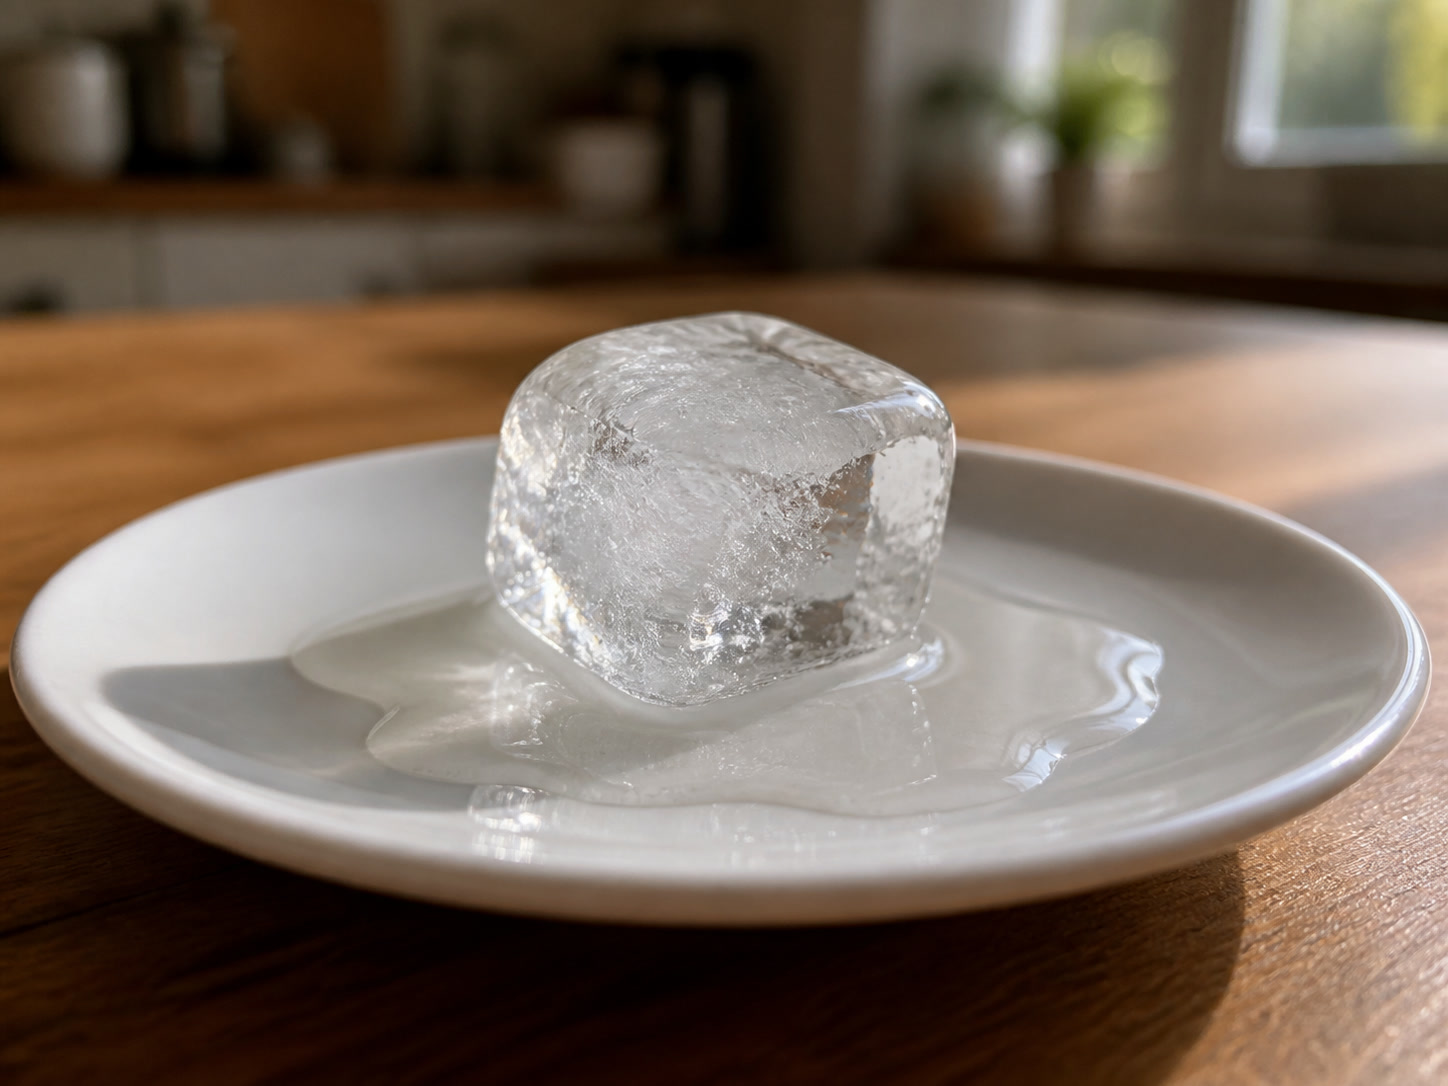
\includegraphics[width=0.52\linewidth]{images/book1/ai/g1-hot-cold-melting-cube.jpg}

{\small El calor en acción: el cubito de hielo de la cocina, sorprendido cuando empieza a derretirse en su charco.}
\end{omfigure}

\begin{example}[El frío también puede ganar]\label{ex:g1:hot-and-cold:freezer}
El congelador hace el trabajo contrario: mete dentro un vasito de agua
por la tarde y por la mañana lo encontrarás duro como una piedra ---
hielo. El calor derrite el hielo y lo convierte en agua; el frío
fuerte convierte el agua otra vez en hielo. El agua seguirá cambiando
de un lado a otro así a lo largo de todo el libro.
\end{example}

\section{Ejercicios}

\begin{exercise}[$\star$]\label{exo:g1:hot-and-cold:1}
Ordena del más frío al más caliente: el agua del baño; \ un cubito de
hielo; \ la sopa recién salida de la olla; \ el aire de tu
habitación.
\end{exercise}

\begin{exercise}[$\star$]\label{exo:g1:hot-and-cold:2}
Encuentra la palabra que compara: el agua del grifo está \dots\
comparada con el chocolate caliente, pero \dots\ comparada con el zumo
de naranja del frigorífico.
\end{exercise}

\begin{exercise}[$\star$]\label{exo:g1:hot-and-cold:3}
Nombra cuatro cosas que calienten lo que tienen cerca. ¿Cuál de ellas
calienta el parque entero?
\end{exercise}

\begin{exercise}[$\star$]\label{exo:g1:hot-and-cold:4}
Frota deprisa las palmas de las manos mientras cuentas hasta $10$ y
tócate después la mejilla. ¿Qué notas? ¿Qué ha hecho el frotamiento?
\end{exercise}

\begin{exercise}[$\star$]\label{exo:g1:hot-and-cold:5}
Dos cubitos de hielo salen juntos del congelador. Uno va a un plato al
sol y el otro a un plato a la sombra. ¿Cuál se derrite antes y por
qué?
\end{exercise}

\begin{exercise}[$\star$]\label{exo:g1:hot-and-cold:6}
¿Qué hay en el charco que queda en el plato después de que se derrita
un cubito de hielo? ¿Adónde se fue el hielo duro?
\end{exercise}

\begin{exercise}[$\star$]\label{exo:g1:hot-and-cold:7}
Un tobogán de metal y un banco de madera han estado a la sombra toda
la mañana. Tomás toca los dos y dice que el tobogán está más frío. Usa
la \cref{rem:g1:hot-and-cold:fooled} para explicar qué pasa en
realidad.
\end{exercise}

\begin{exercise}[$\star$]\label{exo:g1:hot-and-cold:8}
Con el \cref{met:g1:hot-and-cold:compare}, explica cómo averiguar cuál
de dos cuencos de agua está más caliente. ¿Por qué hay que usar la
misma mano para los dos?
\end{exercise}

\begin{exercise}[$\star\star$]\label{exo:g1:hot-and-cold:9}
Lea hace un muñeco de nieve y, como le da pena, lo envuelve en su
abrigo calentito. Su hermano dice que el abrigo lo derretirá más
deprisa. Lea dice que el abrigo lo mantendrá frío más tiempo. ¿Quién
tiene razón y por qué? (Piensa en la
\cref{rem:g1:hot-and-cold:coat}: ¿qué hace de verdad un abrigo?)
\end{exercise}
